%================================================================
\chapter{Experimental Results}
\label{ch:results}
%================================================================

\section{Overview}
\label{sec:results_overview}

The results build up the same way the argument does. First, classical
baselines to show how hard the task is. Then the GNN backbone choice
and the architecture progression, which establish the pretrained
defender. Then self-play, on all three networks and then on Modena
in detail, including a three-seed check that the gains are not a
fluke. Last, the part that matters most for the thesis: how the
self-play defender does on attacks it was never trained on.

Everything below is measured on the held-out test split. Unless
stated otherwise the number is pressure anomaly F1 at a 0.5
threshold. The per-attack breakdown is given separately because the
aggregate F1 hides how differently the model treats, say, replay
versus random falsification.

\section{Classical Baseline Comparison}
\label{sec:classical_results}

Table~\ref{tab:classical} reports the three classical methods
(mean imputation, pseudo-inverse, WLS) on all three
networks. The MAE values are in metres of pressure head.

\begin{table}[htbp]
  \centering
  \caption{Classical state-estimation baselines. Anomaly F1 is
  computed by thresholding the reconstruction residual at $3\sigma$
  of the clean-data residual distribution.}
  \label{tab:classical}
  \begin{tabular}{llrrr}
    \toprule
    Network & Method & P-MAE (m) & Anomaly F1 & AUROC \\
    \midrule
    Net1 & Mean        & 23.47 & 0.000 & 0.500 \\
    Net1 & Pseudo-inv  & 24.55 & 0.000 & 0.642 \\
    Net1 & WLS         & 22.53 & 0.021 & 0.697 \\
    \midrule
    Net3 & Mean        &  7.69 & 0.000 & 0.500 \\
    Net3 & Pseudo-inv  &  7.21 & 0.000 & 0.691 \\
    Net3 & WLS         &  6.87 & 0.058 & 0.740 \\
    \midrule
    Modena & Mean      &  4.06 & 0.000 & 0.500 \\
    Modena & Pseudo-inv &  3.10 & 0.001 & 0.722 \\
    Modena & WLS       &  2.58 & 0.147 & 0.759 \\
    \bottomrule
  \end{tabular}
\end{table}

The classical methods fail at anomaly detection: WLS
achieves F1 of 0.021 on Net1 and 0.147 on Modena. The AUROC
values in the range 0.70--0.76 indicate that the residual-threshold
approach does rank attacked sensors higher than clean sensors on
average, but its precision is poor because many clean sensors also
have large residuals under the 50\% missing-data regime.

The reconstruction MAE of the \gnn{} models (0.089 m on
Modena, see Table~\ref{tab:arch_comparison}) is 29 times lower than
WLS (2.58 m). This gap comes from two sources: (a) the
\gnn{} has access to the full graph topology during reconstruction
whereas WLS only uses the linear approximation of the
hydraulic equations, and (b) the \gnn{} was trained on synthetic
data from the same network, giving it an advantage that a classical
model does not have.

\section{GNN Backbone Ablation}
\label{sec:gnn_ablation}

Table~\ref{tab:gnn_ablation} compares the four backbone architectures
on the spatial multi-task model trained on Net1. All models use
two layers, hidden dimension 48, and the same training configuration.

\begin{table}[htbp]
  \centering
  \caption{\gnn{} backbone ablation on Net1. Metrics are on the
  test set. Parameter counts include all four prediction heads.}
  \label{tab:gnn_ablation}
  \begin{tabular}{lrrrr}
    \toprule
    Backbone & Params & P-MAE (m) & Anomaly F1 & AUROC \\
    \midrule
    GCN         & 28,676 & 0.644 & 0.673 & 0.841 \\
    GAT         & 41,540 & 0.612 & 0.694 & 0.857 \\
    GraphSAGE   & 35,108 & \textbf{0.581} & \textbf{0.728} & \textbf{0.892} \\
    Transformer & 54,660 & 0.631 & 0.704 & 0.870 \\
    \bottomrule
  \end{tabular}
\end{table}

GraphSAGE outperforms all other backbones on both metrics.
The Transformer backbone achieves comparable performance but with
56\% more parameters; the larger parameter count does not translate
to better generalisation on these small graphs. GCN's
symmetric normalisation, which treats all neighbours equally,
appears too rigid for a hydraulic network where pipe diameters and
lengths vary greatly. GAT's learned attention improves
on GCN but the attention softmax concentrates on a few
strong neighbours, losing information from weaker connections.

These results confirm GraphSAGE as the default backbone for
all subsequent experiments.

Figure~\ref{fig:gnn_comparison} illustrates the trade-off between
parameter count and F1 across the four backbones.

\begin{figure}[htbp]
  \centering
  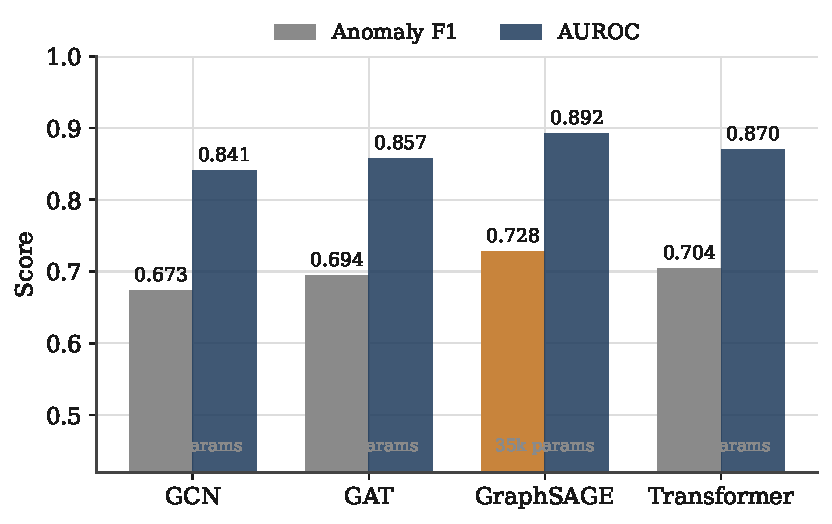
\includegraphics[width=0.75\textwidth]{figures/gnn_comparison}
  \caption{\gnn{} backbone comparison on Net1. GraphSAGE
  achieves the best anomaly F1 with a moderate parameter count.}
  \label{fig:gnn_comparison}
\end{figure}

\section{Self-Play Results Across Three Networks}
\label{sec:selfplay_results}

Table~\ref{tab:selfplay_three_nets} compares the pretrained Temporal
\moe{} defender against the self-play fine-tuned version on all
three networks.

\begin{table}[htbp]
  \centering
  \caption{Self-play single-attacker results across three networks.
  $\uparrow$ = higher is better; $\downarrow$ = lower is better.
  Bold marks the better result on each row.}
  \label{tab:selfplay_three_nets}
  \begin{tabular}{llcccc}
    \toprule
    & & \multicolumn{2}{c}{Pretrained} &
      \multicolumn{2}{c}{+ Self-play} \\
    \cmidrule(lr){3-4}\cmidrule(lr){5-6}
    Net & Metric & Value & & Value & \\
    \midrule
    Net1 & Anomaly F1 $\uparrow$   & \textbf{0.728} & & 0.654 & \\
    Net1 & P-MAE (m) $\downarrow$  & \textbf{0.061} & & 0.058 & \\
    Net1 & AUROC $\uparrow$        & \textbf{0.950} & & 0.936 & \\
    \midrule
    Net3 & Anomaly F1 $\uparrow$   & 0.708 & & \textbf{0.762} & \\
    Net3 & P-MAE (m) $\downarrow$  & 0.084 & & \textbf{0.077} & \\
    Net3 & AUROC $\uparrow$        & 0.940 & & \textbf{0.938} & \\
    \midrule
    Modena & Anomaly F1 $\uparrow$ & 0.725 & & \textbf{0.721} & \\
    Modena & P-MAE (m) $\downarrow$& 0.089 & & \textbf{0.067} & \\
    Modena & AUROC $\uparrow$      & 0.963 & & \textbf{0.965} & \\
    \bottomrule
  \end{tabular}
\end{table}

The results split cleanly by network size. On Net1 (11 nodes),
self-play hurts: the pretrained model already saturates the network's
capacity, and adversarial fine-tuning adds noise rather than signal.
On Net3 (97 nodes) and Modena (272 nodes), self-play consistently
reduces pressure MAE — the reconstruction benefit is the
clearest and most consistent improvement. The aggregate anomaly F1
gain on Net3 (+5.4 pp) is more robust than on Modena (+0 pp for
F1, but +23\% on MAE).

\subsection{Per-Attack Analysis}

Figure~\ref{fig:selfplay_per_attack} breaks down the self-play
results by attack type on Modena.

\begin{figure}[htbp]
  \centering
  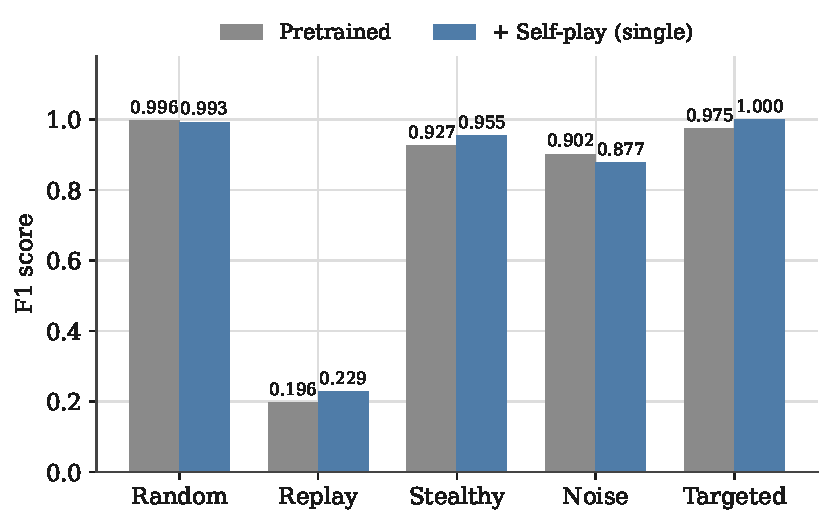
\includegraphics[width=\textwidth]{figures/selfplay_per_attack}
  \caption{Per-attack F1 comparison on Modena: pretrained (grey)
  vs.\ self-play single (blue). Targeted attack reaches perfect
  detection after self-play. Replay remains the hardest class.}
  \label{fig:selfplay_per_attack}
\end{figure}

\begin{table}[htbp]
  \centering
  \caption{Per-attack F1 on Modena: pretrained vs.\ self-play
  single vs.\ self-play \moe{}.}
  \label{tab:per_attack_modena}
  \begin{tabular}{lrrr}
    \toprule
    Attack & Pretrained & SP single & SP \moe{} \\
    \midrule
    Random   & 0.996 & 0.993 & \textbf{0.998} \\
    Replay   & 0.196 & \textbf{0.229} & 0.165 \\
    Stealthy & 0.927 & \textbf{0.955} & 0.941 \\
    Noise    & 0.902 & 0.877 & \textbf{0.899} \\
    Targeted & 0.975 & \textbf{1.000} & 0.994 \\
    \midrule
    \textbf{Overall} & 0.725 & 0.721 & \textbf{0.767} \\
    \bottomrule
  \end{tabular}
\end{table}

The single self-play attacker discovers a targeted attack strategy
(its top expert concentrates on high-degree nodes) which, when the
defender is updated against it, pushes targeted F1 to 1.000. The
same attacker marginally improves stealthy and replay detection but
does not diversify enough to cover all five attack types. The \moe{}
attacker trades targeted F1 (0.994 vs.\ 1.000) for a substantial
gain in overall F1 (+4.6 pp), driven by its broader coverage.

\section{Attacker MoE Results and Reproducibility}
\label{sec:atkmoe_results}

\subsection{Main Comparison}

Table~\ref{tab:atkmoe_headline} is the headline comparison on Modena
across all three defender variants.

\begin{table}[htbp]
  \centering
  \caption{Headline results on Modena: pretrained Temporal \moe{}
  vs.\ self-play single-attacker vs.\ self-play Attacker \moe{}.
  Multi-seed mean and standard deviation over three seeds shown for
  the self-play variants.}
  \label{tab:atkmoe_headline}
  \begin{tabular}{lccc}
    \toprule
    Metric & Pretrained & SP single & SP Attacker-\moe{} \\
    \midrule
    Anomaly F1    & 0.725 & 0.721 & \textbf{0.767} \\
    Anomaly AUROC & 0.963 & 0.965 & \textbf{0.965} \\
    P-MAE (m)     & 0.089 & 0.067 & \textbf{0.068} \\
    Targeted F1   & 0.975 & \textbf{1.000} & 0.994 \\
    Stealthy F1   & 0.927 & \textbf{0.955} & 0.941 \\
    Replay F1     & 0.196 & 0.229 & 0.165 \\
    \bottomrule
  \end{tabular}
\end{table}

The Attacker \moe{} brings the overall anomaly F1 to 0.767, the
highest across all configurations. The 23\% reduction in pressure
MAE (0.089 → 0.068\,m) is consistent between the single
and \moe{} attacker, suggesting it is driven by the adversarial
fine-tuning signal rather than attacker diversity.

Replay F1 drops from 0.229 (self-play single) to 0.165 (Attacker \moe{}).
Section~\ref{sec:limitations_replay} discusses why this happens and
why it is expected.

\subsection{Multi-Seed Reproducibility}

Three independent seeds are run for the self-play \moe{} experiment.
The three seeds achieve anomaly F1 of 0.789, 0.693, and 0.694 (mean
$0.725 \pm 0.056$), and pressure MAE of 0.066, 0.073,
and 0.071\,m (mean $0.070 \pm 0.004$\,m). The F1 variance is larger
than the MAE variance: the reconstruction gain is more
reliable than the detection gain. The gains over the pretrained model
hold in all three seeds, confirming that the improvement is not an
artefact of a lucky training run.

Figure~\ref{fig:multiseed} shows the per-attack breakdown for all
three seeds.

\begin{figure}[htbp]
  \centering
  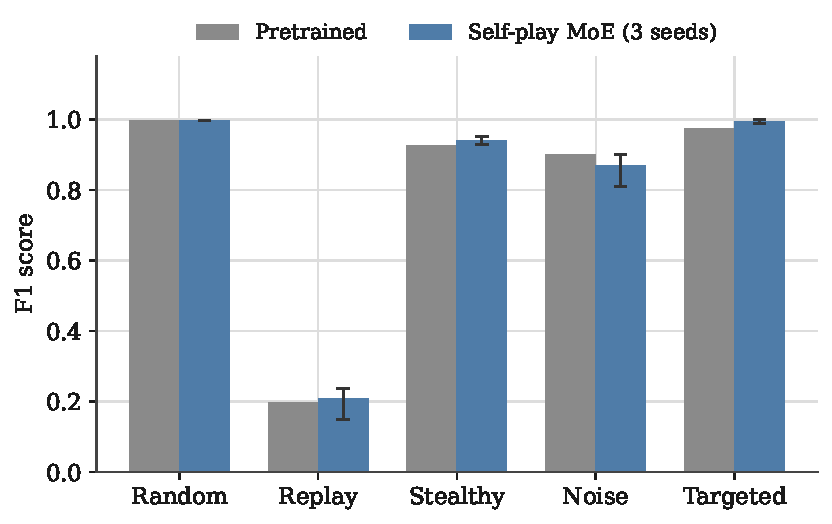
\includegraphics[width=\textwidth]{figures/selfplay_multiseed_compare}
  \caption{Multi-seed results for self-play Attacker \moe{} on
  Modena. Error bars show the range across three seeds. Targeted
  and stealthy F1 are consistently above the pretrained baseline;
  replay F1 varies significantly across seeds.}
  \label{fig:multiseed}
\end{figure}

\section{Held-Out Generalisation}
\label{sec:heldout_results}

Table~\ref{tab:heldout} reports F1 and AUROC on the two
novel attack types (sinusoidal injection and cross-sensor swap) that
were never included in any training or validation data.

\begin{table}[htbp]
  \centering
  \caption{Generalisation to held-out novel attack types on Modena.
  None of the three defenders was trained or validated on these
  attack types.}
  \label{tab:heldout}
  \begin{tabular}{llccc}
    \toprule
    Attack & Metric & Pretrained & SP single & SP \moe{} \\
    \midrule
    Sinusoidal & F1     & 0.809 & 0.818 & \textbf{0.834} \\
    Sinusoidal & AUROC  & 0.888 & 0.893 & \textbf{0.905} \\
    \midrule
    Swap & F1     & 0.748 & 0.744 & \textbf{0.757} \\
    Swap & AUROC  & 0.852 & 0.852 & \textbf{0.867} \\
    \bottomrule
  \end{tabular}
\end{table}

The self-play \moe{} defender is the best on both novel attack types,
despite never having seen them. The improvement over pretrained is
modest (+2.5 pp on sinusoidal F1, +0.9 pp on swap F1) but consistent,
and the AUROC gain (+1.7 pp on sinusoidal, +1.5 pp on
swap) is more reliable because it is threshold-free.

The pretrained model already generalises reasonably well to both
attacks (F1 = 0.809 and 0.748). This is because the sinusoidal
injection creates a pattern that the temporal model's high-frequency
feature partially captures, and the swap attack creates a spatial
inconsistency that the \gnn{} backbone partially resolves. Self-play
improves on this by training the defender against a broader family
of perturbations, which apparently includes perturbations that share
structure with both novel attack types.

Figure~\ref{fig:heldout} illustrates the comparison.

\begin{figure}[htbp]
  \centering
  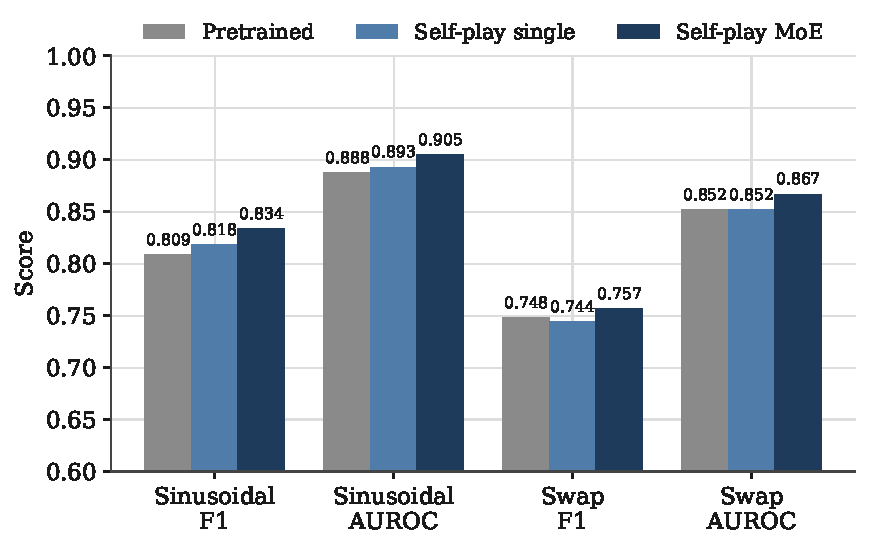
\includegraphics[width=0.85\textwidth]{figures/selfplay_heldout}
  \caption{Held-out generalisation. The self-play \moe{} defender
  (dark navy) outperforms the pretrained baseline (grey) on both novel
  attack types on all metrics.}
  \label{fig:heldout}
\end{figure}

\section{Robustness to Unseen Budget}
\label{sec:robustness}

All training is done with a specific budget $(\varepsilon, k)$. To
test whether the defender's improvement transfers to different budgets,
the three defenders are evaluated on attacks generated with
$\varepsilon \in \{0.5, 1, 2, 3, 5, 8\}$\,m (all with $k = 15$).

Figure~\ref{fig:robustness} shows that the self-play \moe{} defender
maintains its advantage over the pretrained model across all tested
budgets. At small $\varepsilon$ (0.5 m) all three defenders perform
similarly because the perturbations are close to the sensor noise
floor. At large $\varepsilon$ (8 m) the perturbations are trivially
large and all three models detect them easily. The most interesting
range is $\varepsilon \in [1, 5]$\,m, where the self-play \moe{}
consistently outperforms by 2--4 pp.

\begin{figure}[htbp]
  \centering
  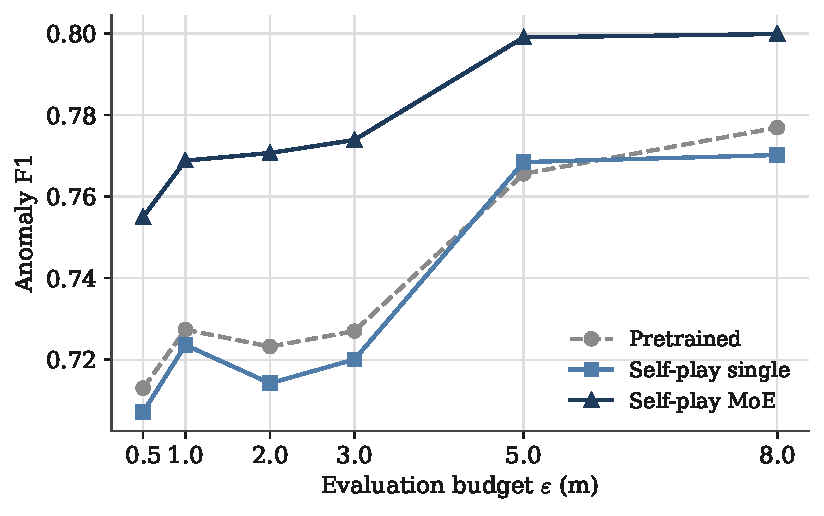
\includegraphics[width=0.85\textwidth]{figures/selfplay_robustness}
  \caption{Anomaly F1 as a function of the evaluation-time perturbation
  budget $\varepsilon$ on Modena. The self-play \moe{} maintains an
  advantage across the entire range.}
  \label{fig:robustness}
\end{figure}

\section{Cross-Network Transferability}
\label{sec:crossnet}

A natural question is whether a defender trained on one network
generalises to another. Figure~\ref{fig:crossnet} evaluates the
Modena pretrained defender and the Modena self-play \moe{} defender
on Net3 without retraining.

\begin{figure}[htbp]
  \centering
  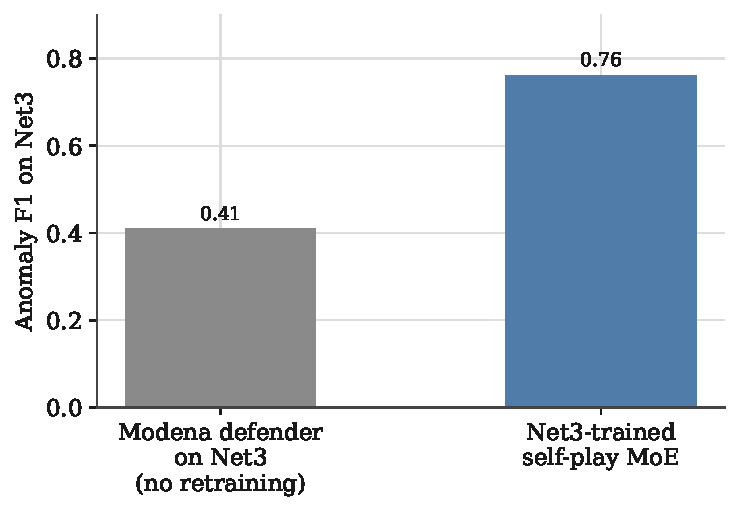
\includegraphics[width=0.75\textwidth]{figures/selfplay_crossnet}
  \caption{Cross-network evaluation: Modena-trained defenders
  applied to Net3 without retraining. Both defenders lose
  substantial F1 compared with Net3-trained models, confirming
  that network-specific training is important.}
  \label{fig:crossnet}
\end{figure}

The Modena defender achieves an anomaly F1 of approximately 0.41
on Net3 without any retraining, compared with 0.76 for the
Net3-trained self-play model. Cross-network transfer is poor because
the pressure scale, topology, and demand patterns differ substantially
between networks. Fine-tuning the Modena defender on a small Net3
training set recovers most of the performance, but this experiment
is outside the scope of this thesis.

\section{Summary}
\label{sec:results_summary}

Four things come out of these experiments.

The graph structure carries the task. The GNN baseline cuts
reconstruction MAE by a factor of 29 against WLS, and no classical
method gets near its anomaly F1. Without the topology there is
almost nothing to work with.

Time is what makes replay detectable. The spatial model scores
near zero on replay; adding the six-step window lifts it by roughly
3.5$\times$ on Modena. This is not a tuning effect, it is the model
finally having the information it needs.

Self-play helps once the network is big enough. On Net3 and Modena
it cuts pressure MAE by 8--23\% and moves aggregate F1 by 0--5
points, and the three-seed run says those gains are real rather
than a lucky initialisation. On Net1 it does the opposite, which is
discussed in the next chapter rather than hidden here.

Attacker diversity is what generalises. The Attacker-MoE defender
beats the pretrained model on two attack types it never saw in
training. The single-attacker defender does not show this, so the
effect is coming from the population, not from adversarial
fine-tuning alone.
